\clearpage\newpage
\subsection{Momentum corrections} 
Drift chamber misalignment and an inaccurate magnetic field map
are the main reasons why the reconstruction of the momentum 
is sligtly incorrect. This is reflected on quantities like 
$W$ or missing mass. For example for elastic events
the $W$ distribution is distorted as seen in \F{fig:w_sec1_before}
where it is plotted against the electron azimuthal angle in the laboratory system after angle corrections.
\begin{figure}[h]
 \begin{center}
 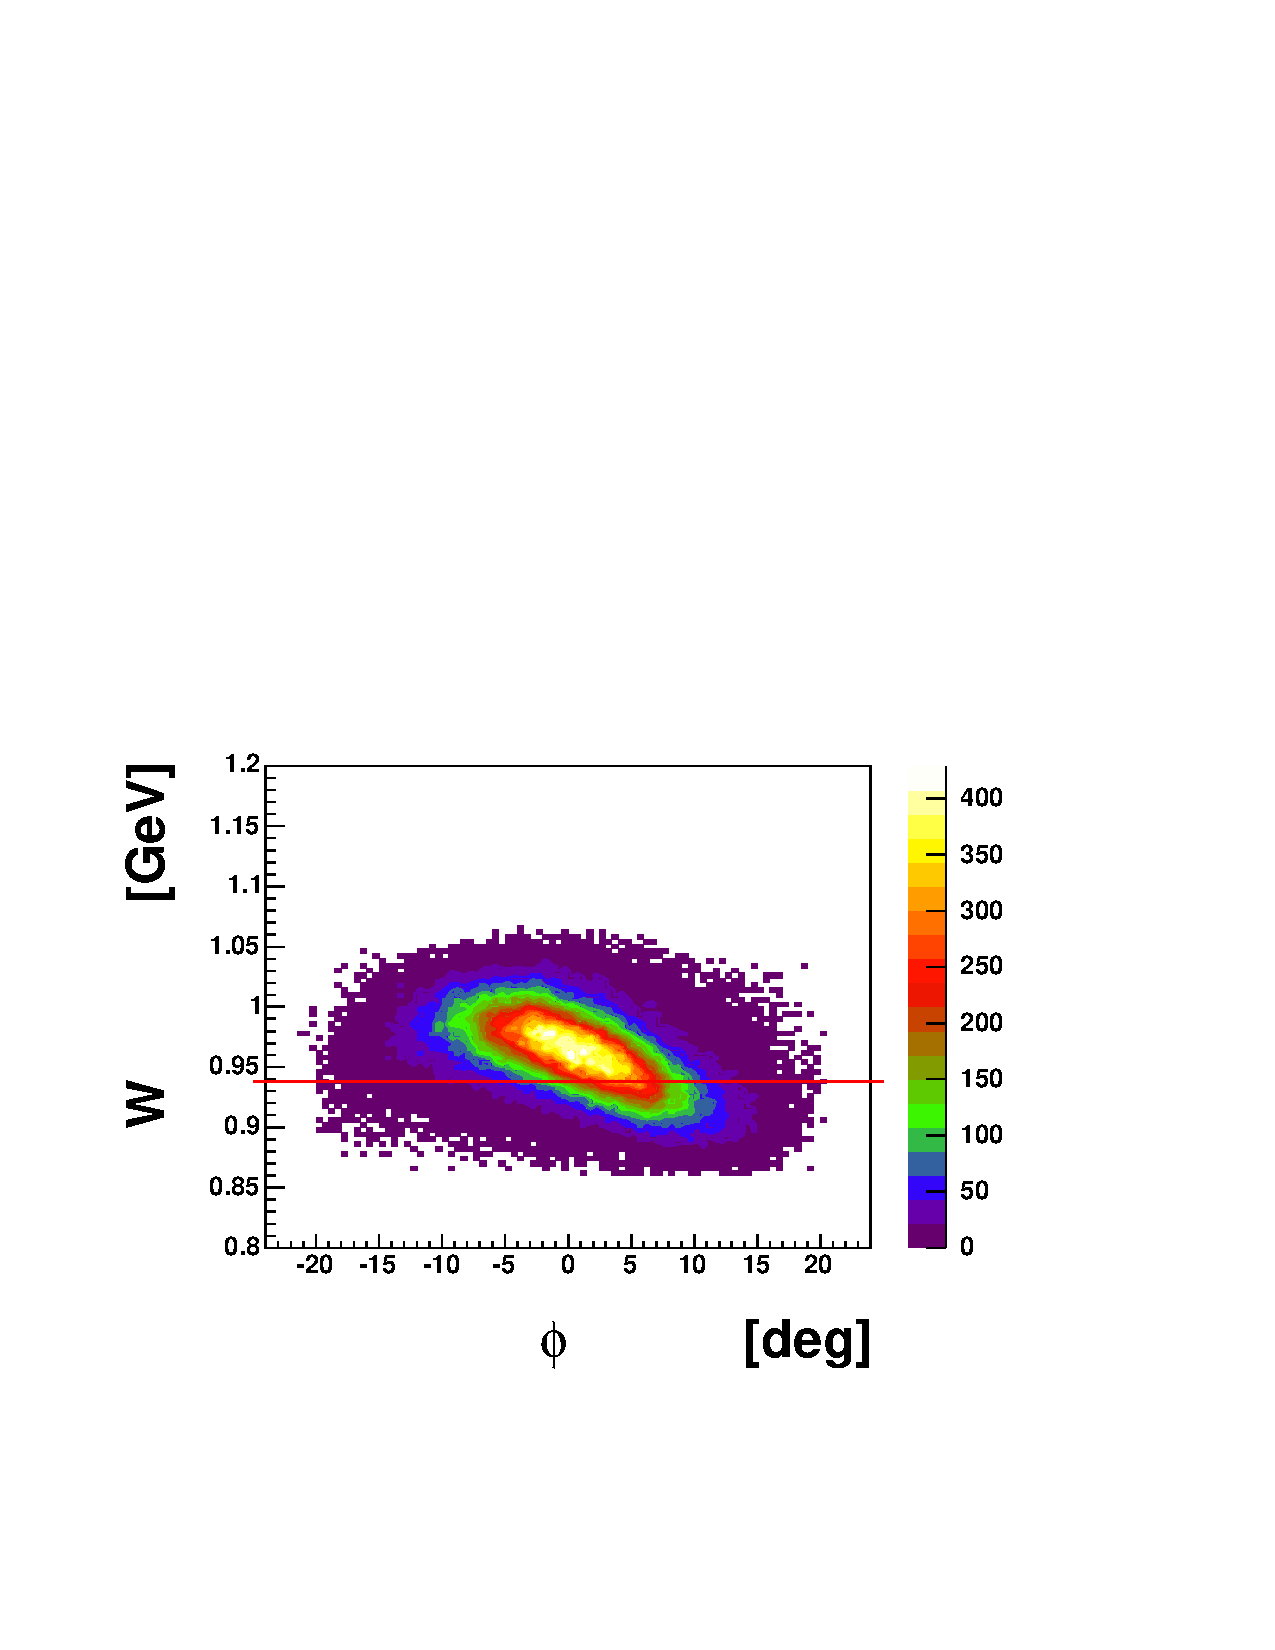
\includegraphics[width = 13cm, bb=0 120 550 480]{data_reduction/kine_corr/img/w_sec1_before}
 
  \caption[$W$ distribution as a function of electron $\phi$ for elastic events after angle corrections]
          { $W$ distribution as a function of electron $\phi$ for elastic events after angle corrections. 
                     The red line is the mass of the proton.}
 \label{fig:w_sec1_before}
 \end{center}
\end{figure}

The distortion turns out to depend upon $\phi$ and $\theta$ of the electron (and not on its momentum).
Recall that for elastic events the $\theta$ and the momentum $p$ are highly correlated\footnote{This is not true for other reactions,
where the distortion is also momentum dependent.}.
Such distortion is sector dependant and needs to be corrected.

The empirical correction discussed below  is based upon the elastic kinematics
The mass of the $\Delta(1232)$ is close enough to the one of the proton to fairly justify applying
the correction for pion electroproduction in the $\Delta$ region because the phase spaces do not differ a lot. \\
The quantity
$$
 \Delta p = p_{meas} - p_{calc} = p_{meas} - \Dfrac{E}{(1+E(1-\cos\theta)/M_P)}
$$
where $E$ is the beam energy, is extracted and plotted versus $\phi$ for different $\theta$ slices  
in \F{fig:corr_e_fits} for sector 3. $\Delta p$ is the wanted correction.
Notice that $\Delta p$ depends only upon the scattered electron angle.


Each $\Delta p$ distribution is fitted with a third order polynomial, giving the parameters as a function of $\theta$:
\begin{equation}
a = a(\theta)\, , \,\, 
b = b(\theta)\, , \,\,  
c = c(\theta)\, , \,\,  
d = d(\theta)
\label{eqn:mom_pars}
\end{equation}
Each parameter is then fitted with a $10$th order polynomial to exploit the $\theta$ dependance.
The fits for sector 3 are shown in \F{fig:corr_e_par_fits}.
\begin{figure}[h]
 \begin{center}
 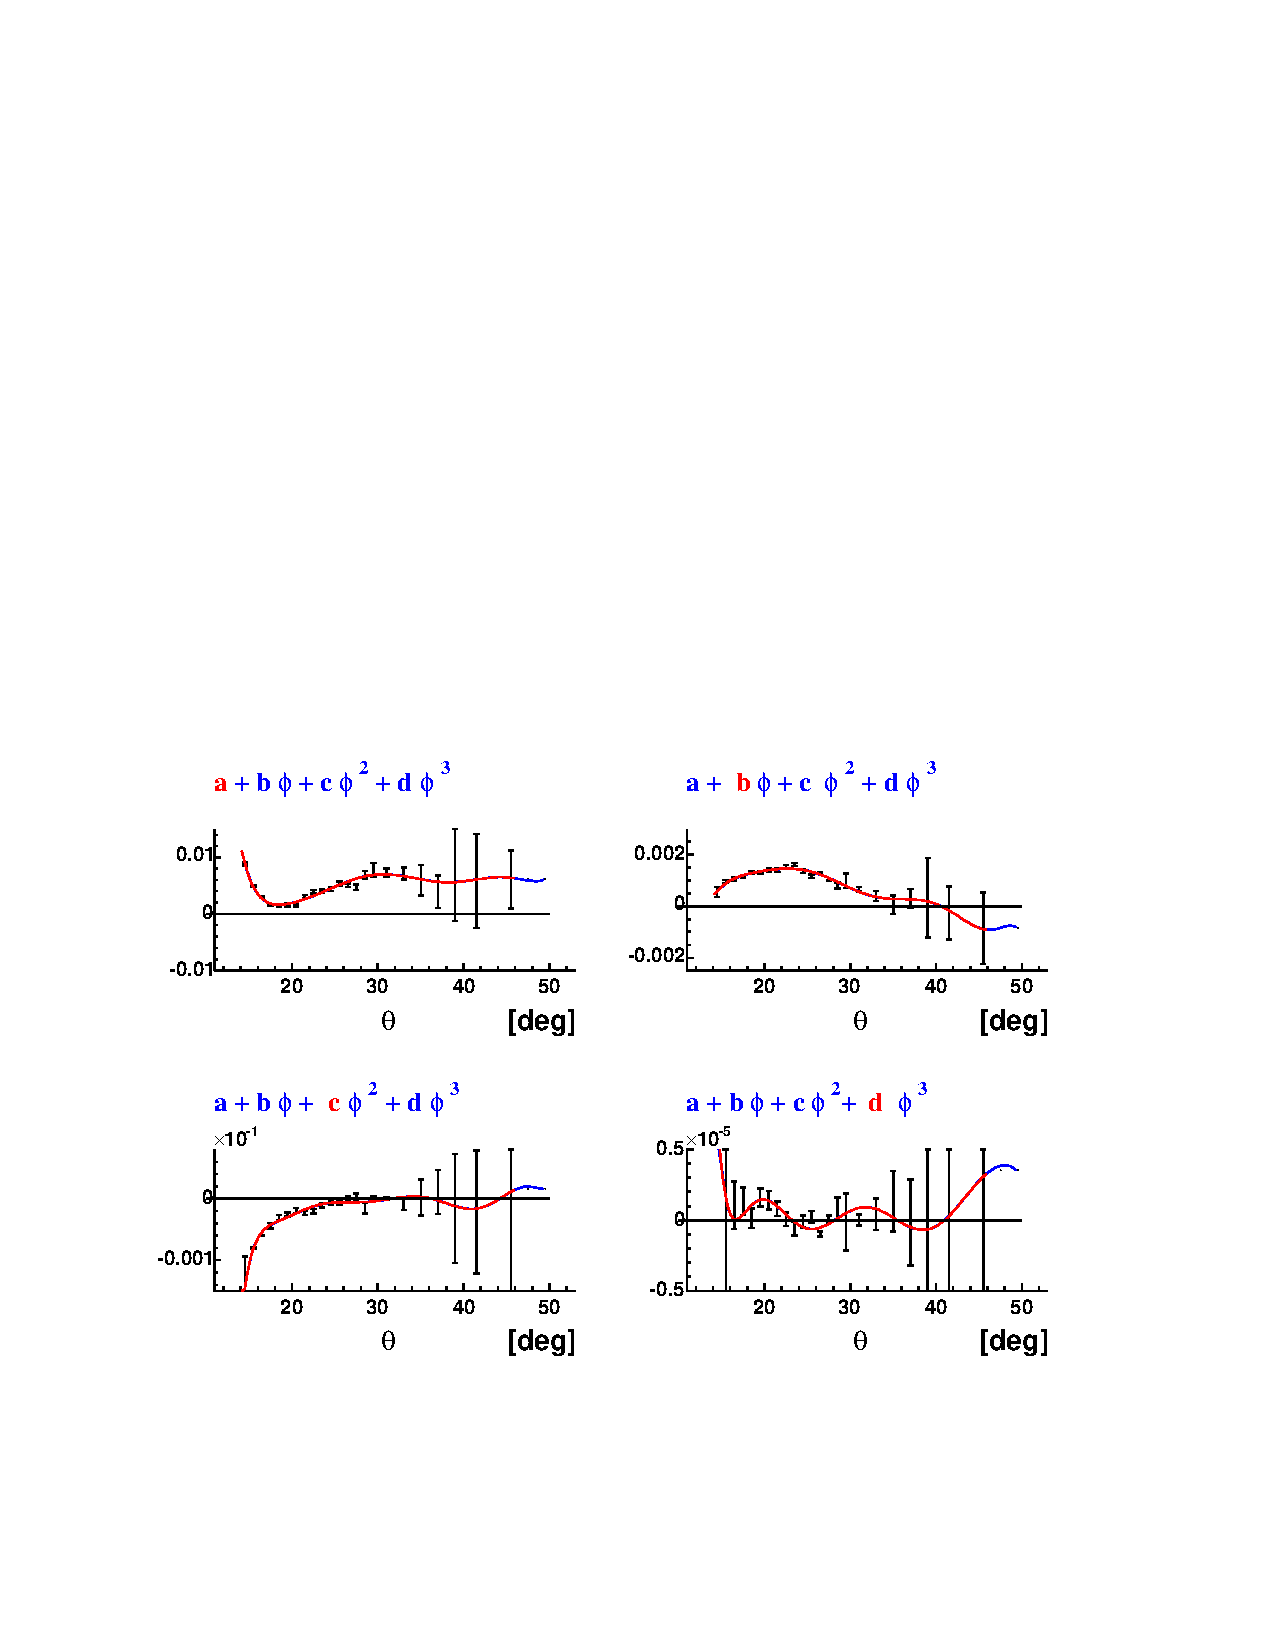
\includegraphics[width = 12cm, bb=60 130 540 450]{data_reduction/kine_corr/img/PART_m}
  \caption[Fits of the third order polynomial parameters as a function of $\theta$ for sector 3]
          { Fits of the third order polynomial parameters as a function of $\theta$ for sector 3.}
 \label{fig:corr_e_par_fits}
 \end{center}
\end{figure}

The overall correction is
$$
\Delta p = a(\theta) + b(\theta)\,\phi + c(\theta)\,\phi^2 + d(\theta)\,\phi^3
$$


\begin{figure}
 \begin{center}
 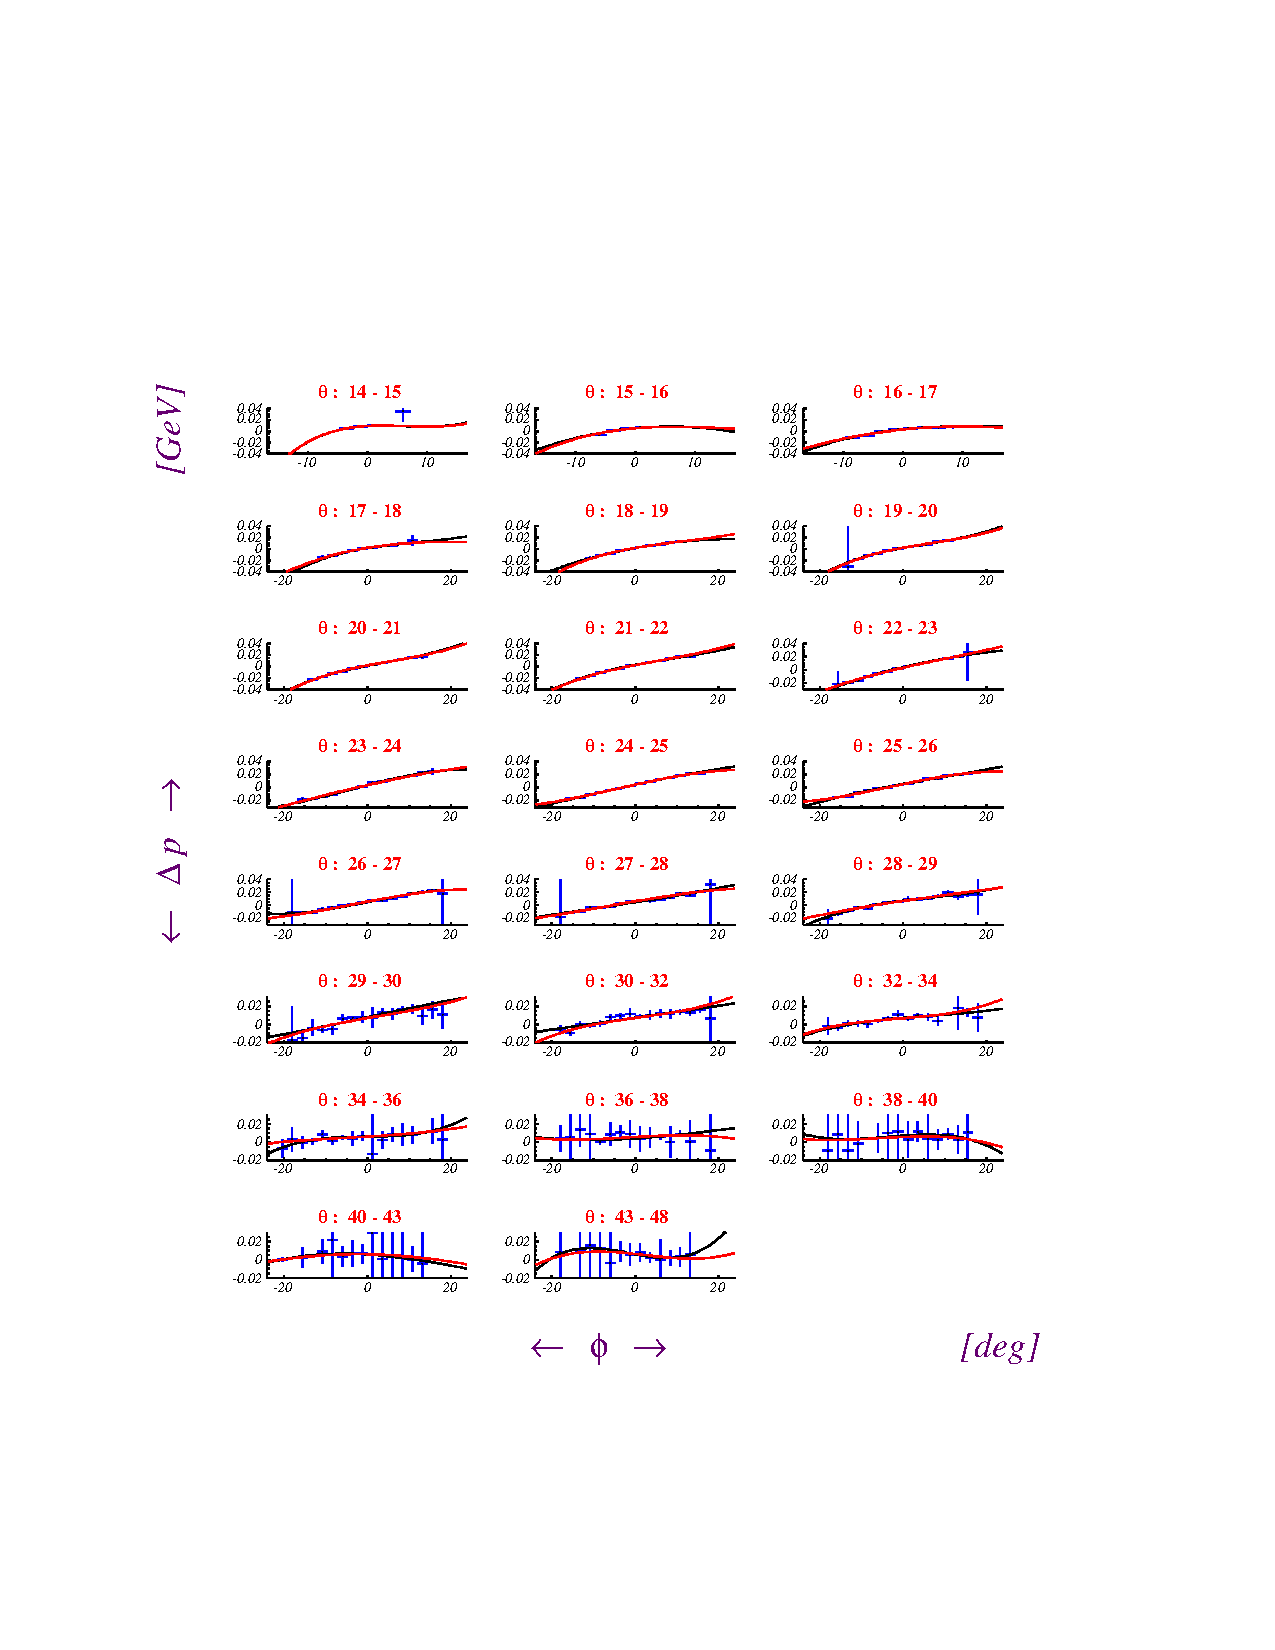
\includegraphics[width = 15cm, bb=70 120 500 640]{data_reduction/kine_corr/img/PHE_m}
  \caption[Fits of the $\Delta p$ distributions for different $\theta$ slices as a function of $\phi$]
          { Fits of the $\Delta p$ distributions for different $\theta$ slices as a function
                     of $\phi$. The black curve
                     is the local fit to the distribution while the red one is the function coming from the 
		     global parameters \ref{eqn:mom_pars}. The procedures make sure that these two curves are close
		     to each other.}
 \label{fig:corr_e_fits}
 \end{center}
\end{figure}
\cia

The result of the correction for sector 1 is shown  in \F{fig:corr_e_result}. One can see that the 
distortion disappeared and the $W$ distribution is now centered at the mass of the proton.
Similar effects are seen for all sectors.
\begin{figure}[h]
 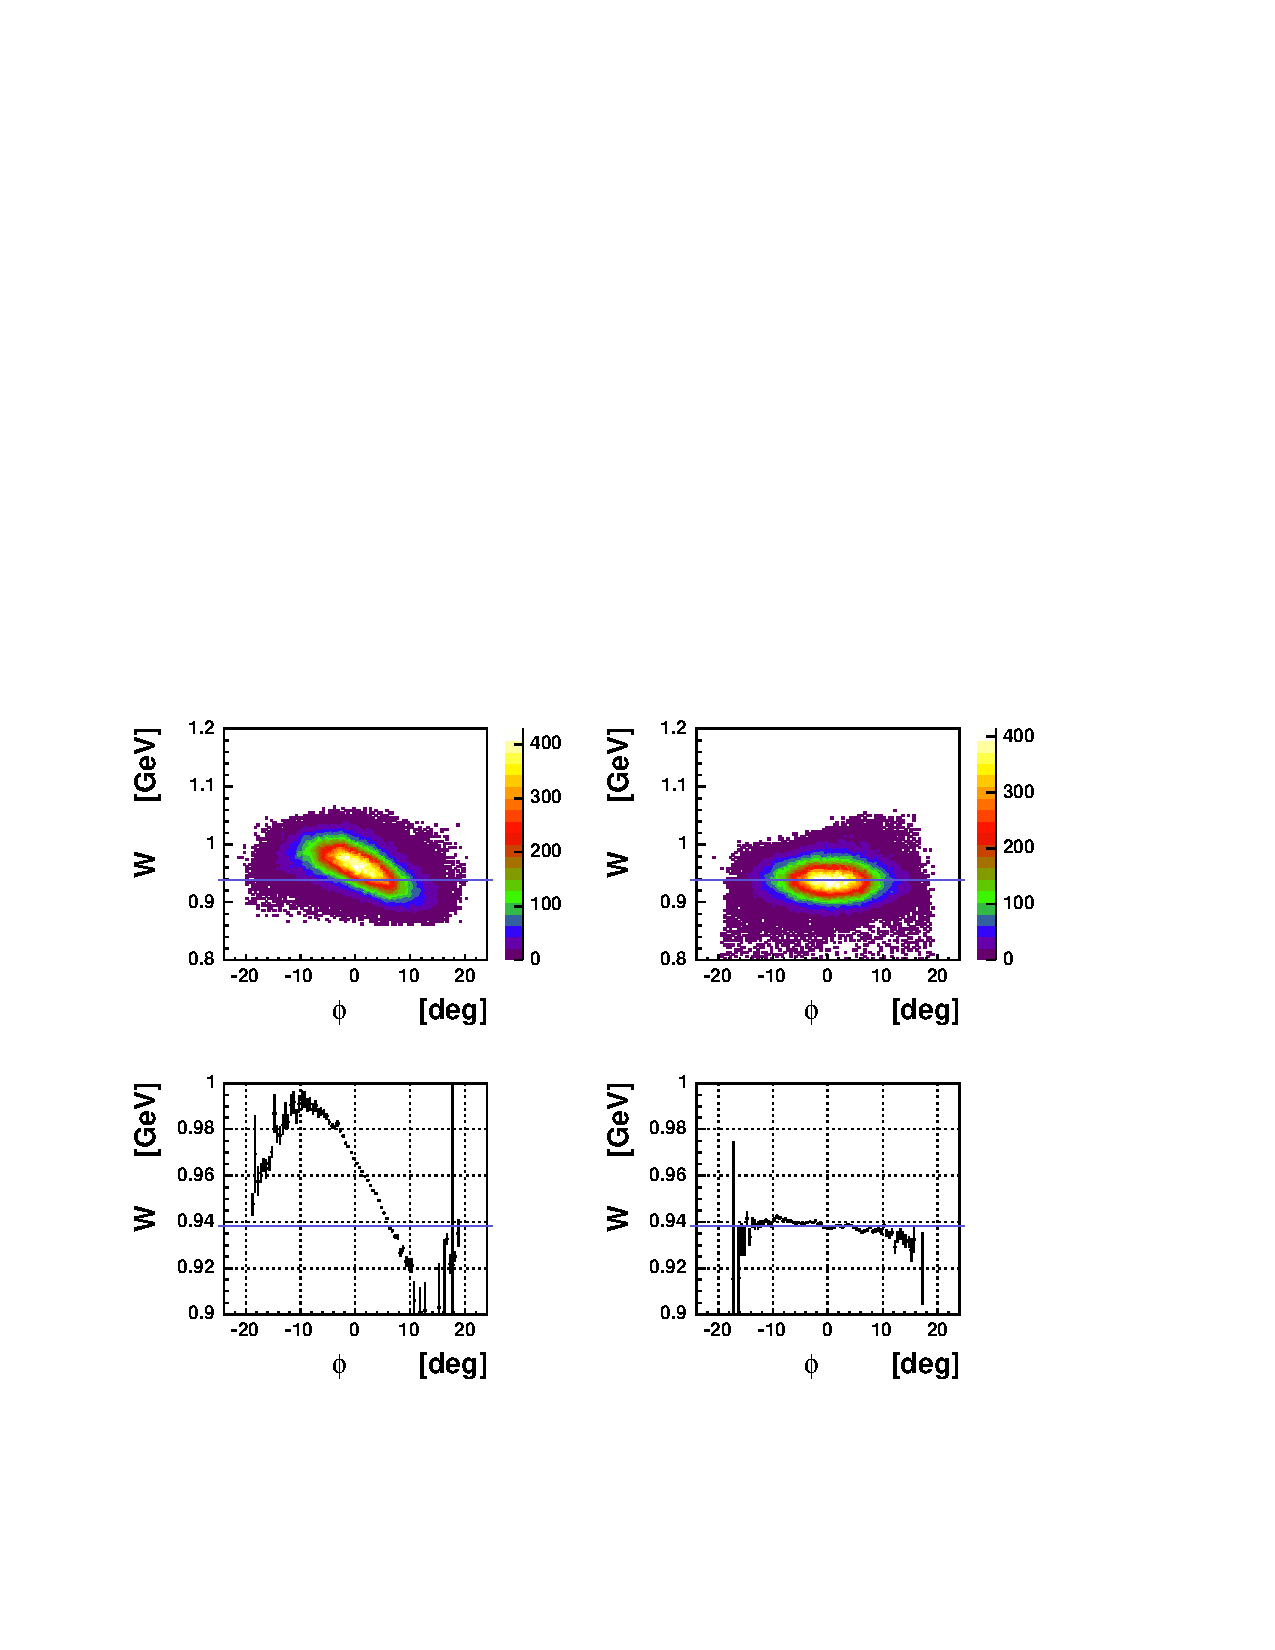
\includegraphics[width = 14.4cm, bb=40 100 500 500]{data_reduction/kine_corr/img/corr_e_result} 
  \caption[The $W$ versus $\phi$ distribution for electrons in sector 1 before (left) and after (right) momentum correction]
          { The $W$ versus $\phi$ distribution for electrons in sector 1  
                     before (left) and after (right)  momentum correction. 
		     The bottom plots are the means of the top distributions sliced along $W$.}
 \label{fig:corr_e_result}
\end{figure}






